\documentclass{article}

\usepackage{tikz}
\usetikzlibrary{automata, positioning, arrows}

\begin{document}

\begin{figure}[ht]
\begin{center}
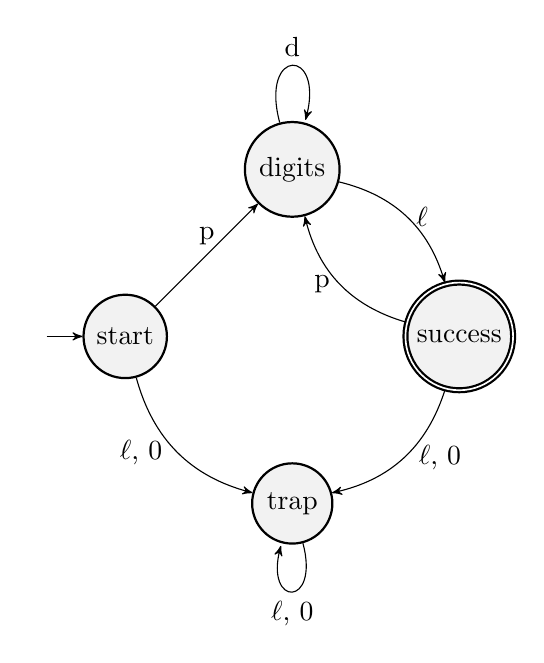
\begin{tikzpicture}
[->,
 >=stealth',
 node distance=3cm,
 every state/.style={thick,fill=gray!10,
 initial text=$$},
]

\node[state]                                    (digits) {digits};
\node[state, initial, below left of=digits]     (start) {start};
\node[state, below right of=start]              (trap) {trap};
\node[state, below right of=digits, accepting]  (success) {success};

\draw
(start)    edge[bend right, left]   node[left=2pt]{$\ell$, 0} (trap)
(start)    edge[above]              node{p} (digits)
(digits)   edge[loop above]         node{d} (digits)
(digits)   edge[bend left, right]   node{$\ell$} (success)
(success)  edge[bend left, left]    node{p} (digits)
(success)  edge[bend left, below]   node[right=2pt]{$\ell$, 0} (trap)
(trap)     edge[loop below]         node{$\ell$, 0} (trap);
\end{tikzpicture}
\end{center}
\end{figure}

\end{document}